\clearpage
\cleardoublepage

\chapter{Transformer架构}

\section{引言}

Transformer架构，由 \cite{vaswani2017attention} 引入，从根本上改变了序列建模和表示学习的格局。通过用自注意力机制取代循环，Transformer实现了跨整个序列的并行计算，显著提高了训练效率，并使得扩展到数十亿参数成为可能。

本章提供Transformer架构的全面论述，从基本的注意力机制到现代大型语言模型。

\section{注意力机制}

\subsection{背景：RNN的局限性}

在Transformer出现之前，序列模型依赖于循环神经网络（RNN）及其变体（LSTM、GRU）。虽然有效，但RNN存在以下问题：
\begin{itemize}
    \item \textbf{顺序计算：}无法跨时间步并行化
    \item \textbf{长程依赖：}通过许多步骤的梯度传播导致梯度消失/爆炸
    \item \textbf{计算效率低：}每个时间步需要从内存加载隐藏状态
\end{itemize}

\subsection{缩放点积注意力}

基本构建块是缩放点积注意力：

\begin{equation}
\text{Attention}(\mathbf{Q}, \mathbf{K}, \mathbf{V}) = \text{softmax}\left(\frac{\mathbf{Q}\mathbf{K}^T}{\sqrt{d_k}}\right)\mathbf{V}
\label{eq:attention}
\end{equation}

其中：
\begin{itemize}
    \item $\mathbf{Q} \in \mathbb{R}^{n \times d_k}$：查询矩阵
    \item $\mathbf{K} \in \mathbb{R}^{m \times d_k}$：键矩阵
    \item $\mathbf{V} \in \mathbb{R}^{m \times d_v}$：值矩阵
    \item $d_k$：键的维度（也是查询维度）
\end{itemize}

\begin{note}[为什么要缩放？]
缩放因子$\sqrt{d_k}$防止点积变得很大，否则会推动softmax进入梯度极小的区域。当$d_k$很大时，点积往往很大，导致softmax饱和（输出接近独热）。
\end{note}

\subsection{自注意力}

自注意力是将注意力应用于查询、键和值都来自同一源的序列：

\begin{equation}
\mathbf{X}_{\text{out}} = \text{Attention}(\mathbf{X}\mathbf{W}_Q, \mathbf{X}\mathbf{W}_K, \mathbf{X}\mathbf{W}_V)
\end{equation}

其中$\mathbf{W}_Q, \mathbf{W}_K, \mathbf{W}_V$是学习的投影矩阵。

关键特性：
\begin{itemize}
    \item \textbf{全到全连接：}每个位置可以关注所有其他位置
    \item \textbf{恒定路径长度：}信息以$O(1)$步流动，与距离无关
    \item \textbf{计算复杂度：}对于序列长度$n$和维度$d$为$O(n^2 \cdot d)$
\end{itemize}

\section{多头注意力}

不是执行单一的注意力函数，而是用学习的线性投影将查询、键和值投影$h$次：

\begin{equation}
\text{MultiHead}(\mathbf{Q}, \mathbf{K}, \mathbf{V}) = \text{Concat}\left(\text{head}_1, \ldots, \text{head}_h\right)\mathbf{W}^O
\end{equation}

其中每个头是：
\begin{equation}
\text{head}_i = \text{Attention}\left(\mathbf{Q}\mathbf{W}_i^Q, \mathbf{K}\mathbf{W}_i^K, \mathbf{V}\mathbf{W}_i^V\right)
\end{equation}

典型配置：$h = 8$个头，$d_k = d_v = d_{\text{model}}/h$。

\begin{properties}[多头注意力的优势]
\begin{itemize}
    \item 每个头可以关注表示的不同方面
    \item 不同的头可能专门处理：位置、句法、语义信息
    \item 模型可以联合关注来自不同表示子空间的信息
\end{itemize}
\end{properties}

\section{Transformer架构}

\subsection{前馈网络}

每层包括一个位置前馈网络：
\begin{equation}
\text{FFN}(\mathbf{x}) = \mathbf{W}_2 \, \sigma\left(\mathbf{W}_1 \mathbf{x} + \mathbf{b}_1\right) + \mathbf{b}_2
\end{equation}

通常实现为两个带ReLU激活的线性变换。内层维度通常为$4 \times d_{\text{model}}$。

\subsection{层归一化}

层归一化通过归一化激活来稳定训练：
\begin{equation}
\mathbf{y} = \frac{\mathbf{x} - \mu}{\sqrt{\sigma^2 + \epsilon}} \odot \gamma + \beta
\end{equation}
其中$\mu = \frac{1}{d}\sum_{i=1}^d x_i$，$\sigma^2 = \frac{1}{d}\sum_{i=1}^d (x_i - \mu)^2$。

存在两种变体：
\begin{itemize}
    \item \textbf{后LN（原始）：}残差连接后的LayerNorm
    \item \textbf{前LN：}在注意力/FFN之前的LayerNorm（对深度网络更稳定）
\end{itemize}

\subsection{残差连接}

每个子层都有一个残差连接：
\begin{equation}
\mathbf{x}_{\text{out}} = \mathbf{x} + \text{SubLayer}(\mathbf{x})
\end{equation}

这使得梯度可以通过跳跃连接流动，并允许网络在有益时学习恒等映射。

\begin{figure}[htbp]
    \centering
    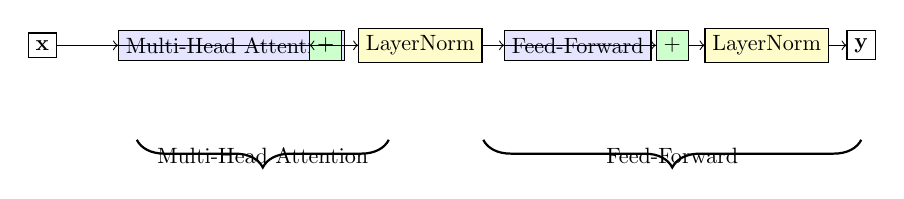
\begin{tikzpicture}[scale=0.8, every node/.style={scale=0.8}]
        % Input
        \node[draw, rectangle] (input) at (0, 0) {$\mathbf{x}$};
        
        % Multi-Head Attention
        \node[draw, rectangle, minimum width=2cm, fill=blue!10] (mha) at (3, 0) {Multi-Head Attention};
        \node[draw, rectangle, fill=green!20] (add1) at (4.5, 0) {$+$};
        \node[draw, rectangle, fill=yellow!20] (ln1) at (6, 0) {LayerNorm};
        
        % FFN
        \node[draw, rectangle, minimum width=2cm, fill=blue!10] (ffn) at (8.5, 0) {Feed-Forward};
        \node[draw, rectangle, fill=green!20] (add2) at (10, 0) {$+$};
        \node[draw, rectangle, fill=yellow!20] (ln2) at (11.5, 0) {LayerNorm};
        
        % Output
        \node[draw, rectangle] (output) at (13, 0) {$\mathbf{y}$};
        
        % Arrows
        \draw[->] (input) -- (mha);
        \draw[->] (mha) -- (add1);
        \draw[->] (add1) -- (ln1);
        \draw[->] (ln1) -- (ffn);
        \draw[->] (ffn) -- (add2);
        \draw[->] (add2) -- (ln2);
        \draw[->] (ln2) -- (output);
        
        % Skip connections
        \draw[-] (input) to[out=0, in=180] (add1);
        \draw[-] (ln1) to[out=0, in=180] (add2);
        
        % Bracket
        \draw[decorate, decoration={brace, amplitude=10pt, mirror}, thick] (1.5, -1.5) -- (5.5, -1.5) node[below, midway] {Multi-Head Attention};
        \draw[decorate, decoration={brace, amplitude=10pt, mirror}, thick] (7, -1.5) -- (13, -1.5) node[below, midway] {Feed-Forward};
    \end{tikzpicture}
    \caption{带残差连接和层归一化的Transformer层。}
    \label{fig:transformer_layer}
\end{figure}

\section{位置编码}

由于自注意力是排列不变的（对输入顺序不变），我们必须注入位置信息：

\begin{equation}
\text{PE}_{(pos, 2i)} = \sin\left(\frac{pos}{10000^{2i/d_{\text{model}}}}\right)
\end{equation}
\begin{equation}
\text{PE}_{(pos, 2i+1)} = \cos\left(\frac{pos}{10000^{2i/d_{\text{model}}}}\right)
\end{equation}

其中$pos$是位置，$i$是维度。

\begin{properties}[位置编码特性]
\begin{itemize}
    \item \textbf{线性关系：} $\text{PE}(pos+k)$可以表示为$\text{PE}(pos)$的线性函数
    \item \textbf{泛化：}可以编码超出训练序列长度的位置
    \item \textbf{相对位置：}旋转位置嵌入（RoPE）在注意力计算中更直接地编码相对位置
\end{itemize}
\end{properties}

替代方案：旋转位置嵌入（RoPE） \cite{su2021roformer}用于LLaMA和GPT-NeoX，在注意力计算中更直接地编码相对位置。

\section{编码器-解码器架构}

原始Transformer使用编码器-解码器结构：

\begin{itemize}
    \item \textbf{编码器：} $N$个处理输入序列的相同层
    \item \textbf{解码器：} $N$个带跨编码器输出的交叉注意力的相同层
    \item \textbf{交叉注意力：}解码器的查询关注编码器的键/值
\end{itemize}

\begin{code}
    \captionof{listing}{PyTorch多头注意力实现}
    \label{code:mha_pytorch_ch12}
\begin{lstlisting}[language=python]
import torch
import torch.nn as nn
import torch.nn.functional as F
import math

class MultiHeadAttention(nn.Module):
    def __init__(self, d_model, num_heads):
        super().__init__()
        assert d_model % num_heads == 0
        
        self.d_model = d_model
        self.num_heads = num_heads
        self.d_k = d_model // num_heads
        
        self.W_q = nn.Linear(d_model, d_model)
        self.W_k = nn.Linear(d_model, d_model)
        self.W_v = nn.Linear(d_model, d_model)
        self.W_o = nn.Linear(d_model, d_model)
    
    def split_heads(self, x, batch_size):
        """Split the last dimension into num_heads."""
        x = x.view(batch_size, -1, self.num_heads, self.d_k)
        return x.permute(0, 2, 1, 3)  # (batch, heads, seq, d_k)
    
    def forward(self, query, key, value, mask=None):
        batch_size = query.size(0)
        
        # Linear projections
        Q = self.W_q(query)
        K = self.W_k(key)
        V = self.W_v(value)
        
        # Split heads
        Q = self.split_heads(Q, batch_size)
        K = self.split_heads(K, batch_size)
        V = self.split_heads(V, batch_size)
        
        # Scaled dot-product attention
        scores = torch.matmul(Q, K.transpose(-2, -1)) / math.sqrt(self.d_k)
        
        if mask is not None:
            scores = scores.masked_fill(mask == 0, -1e9)
        
        attention_weights = F.softmax(scores, dim=-1)
        attention_output = torch.matmul(attention_weights, V)
        
        # Concatenate heads
        attention_output = attention_output.permute(0, 2, 1, 3).contiguous()
        attention_output = attention_output.view(batch_size, -1, self.d_model)
        
        # Final linear projection
        output = self.W_o(attention_output)
        
        return output, attention_weights
\end{lstlisting}
\end{code}

\section{Vision Transformer（ViT）}

Vision Transformer \cite{dosovitskiy2020image}通过将图像块作为令牌来处理，将Transformer架构应用于图像分类：

\begin{enumerate}
    \item 将图像分割为$16 \times 16$块
    \item 展平每个块并投影到$d_{\text{model}}$维度
    \item 添加[CLS]令牌（用于分类）和位置嵌入
    \item 通过标准Transformer编码器处理
    \item 使用最终层的[CLS]令牌输出进行分类
\end{enumerate}

计算复杂度：$O(n^2)$，其中$n = \frac{H \times W}{P^2}$是块的数量。

\section{大型语言模型}

\subsection{GPT架构}

GPT（生成式预训练Transformer）\cite{radford2019language,brown2020language}使用仅解码器架构：
\begin{itemize}
    \item 因果（掩码）自注意力防止关注未来令牌
    \item 语言建模目标：预测下一个令牌
    \item 在大型文本语料库上预训练，然后微调
\end{itemize}

GPT-3扩展到1750亿参数，展示了涌现能力。

\subsection{BERT架构}

BERT \cite{devlin2018bert}使用带双向注意力的仅编码器架构：
\begin{itemize}
    \item 掩码语言建模（MLM）：预测掩码令牌
    \item 下一句预测（NSP）：预测一个句子是否跟随另一个句子
    \item 实现深度双向表示
\end{itemize}

\subsection{现代LLM}

现代大型语言模型结合了几项创新：

\begin{table}[ht]
    \centering
    \caption{现代LLM架构比较}
    \begin{tabular}{L{2.5cm} L{3cm} L{3cm} L{3cm}}
        \toprule
        \textbf{模型} & \textbf{架构} & \textbf{位置编码} & \textbf{关键特性} \\
        \midrule
        GPT-2 & 仅解码器 & 学习到的 & Unigram分词 \\
        GPT-3 & 仅解码器 & 学习到的 & 上下文学习 \\
        LLaMA & 仅解码器 & RoPE & 高效架构 \\
        ChatGLM & Prefix-LM & RoPE & 双语预训练 \\
        Mistral & 仅解码器 & RoPE & 分组查询注意力 \\
        \bottomrule
    \end{tabular}
\end{table}

关键架构差异：
\begin{itemize}
    \item \textbf{RoPE（旋转位置嵌入）：}在旋转矩阵中编码位置，对相对位置更好
    \item \textbf{分组查询注意力（GQA）：}多个查询头共享键/值头，减少内存
    \item \textbf{SwiGLU激活：}用于LLaMA \cite{touvron2023llama}，比GeGLU更好
    \item \textbf{Flash Attention：}IO感知的精确注意力算法 \cite{dao2022flashattention}，将内存从$O(n^2)$减少到$O(n)$
\end{itemize}

\section{效率考量}

\subsection{注意力复杂度}

标准注意力在序列长度上有$O(n^2)$复杂度，对于长序列变得难以承受：

\begin{itemize}
    \item \textbf{Flash Attention：}近似注意力与IO感知，2-4倍加速
    \item \textbf{稀疏注意力：}仅关注位置的子集（Longformer、BigBird）
    \item \textbf{线性注意力：}基于核的近似，复杂度$O(n)$（Performer）
    \item \textbf{低秩注意力：}分解注意力矩阵（Linformer）
\end{itemize}

\subsection{内存优化}

对于大型模型，内存变得至关重要：
\begin{itemize}
    \item \textbf{梯度检查点：}以计算换内存
    \item \textbf{混合精度：}FP16/BF16训练减少2倍内存
    \item \textbf{量化：}INT8/INT4用于推理
    \item \textbf{分页注意力：}KV缓存的内存分页（vLLM）
\end{itemize}

\section{章节小结}

\begin{enumerate}
    \item 自注意力实现并行计算，以$O(1)$路径长度捕获长程依赖
    \item 带$\sqrt{d_k}$缩放的缩放点积注意力防止梯度饱和
    \item 多头注意力允许关注不同的表示子空间
    \item 残差连接和层归一化实现深度网络的稳定训练
    \item 由于注意力是排列不变的，Transformer必须注入位置信息
    \item Vision Transformer（ViT）通过块嵌入将Transformer架构应用于图像
    \item 现代LLM（GPT、BERT、LLaMA）将Transformer扩展到数十亿参数
    \item 效率技术（Flash Attention、稀疏注意力、量化）实现大型模型的实用部署
\end{enumerate}

\section{延伸阅读}

\begin{itemize}
    \item \cite{vaswani2017attention} --- Attention Is All You Need（原始Transformer论文）
    \item \cite{devlin2018bert} --- BERT: 深度双向Transformer的语言理解预训练
    \item \cite{radford2019language} --- 语言模型是无监督多任务学习器（GPT-2）
    \item \cite{brown2020language} --- 语言模型是少样本学习器（GPT-3）
    \item \cite{dosovitskiy2020image} --- 一张图值16x16个词：大规模图像识别的Transformer（ViT）
    \item \cite{su2021roformer} --- RoFormer: 带旋转位置嵌入的增强Transformer
    \item \cite{dao2022flashattention} --- FlashAttention: 带IO感知的快速内存高效精确注意力
    \item \cite{hoffmann2022training} --- 训练计算最优大型语言模型（Chinchilla缩放定律）
    \item \cite{wei2022emergent} --- 大型语言模型的涌现能力
    \item \cite{touvron2023llama} --- LLaMA: 开放高效的基础语言模型
\end{itemize}

\section{练习题}

\begin{enumerate}
    \item \textbf{注意力矩阵形状：}对于序列长度$n=128$、模型维度$d_{model}=512$和8个头，$\mathbf{Q}$、$\mathbf{K}$和$\mathbf{V}$每个头的形状是什么？

    \item \textbf{为什么要按$\sqrt{d_k}$缩放？}当点积变得非常大时，解释softmax分布会发生什么。

    \item \textbf{位置编码：}为什么Transformer必须注入位置信息，而RNN不需要单独的位置编码机制？

    \item \textbf{ViT令牌：} $224\times224$图像被分割为$14\times14$块。在添加[CLS]令牌后，Transformer处理多少个令牌？

    \item \textbf{编码器 vs. 解码器：}从掩码模式、架构类型和预训练目标比较BERT和GPT。

    \item \textbf{效率权衡：}为什么Flash Attention可以加速精确注意力而不改变注意力操作的数学结果？
\end{enumerate}
